%!TeX program = xelatex
\documentclass[12pt,a4paper]{article}
\usepackage{ZJUTReportEN}
\usepackage{listings}
\usepackage{xcolor}

\usepackage{setspace}
\setstretch{1.5} % Set global line spacing to 1.5 times

\usepackage{enumitem} % Load enumitem package to customize list environments
\setlist[itemize]{itemsep=0pt, parsep=0pt} % Set item spacing and paragraph spacing in itemize environment

\setmainfont{Times New Roman} % Set English main text font to Times New Roman

% Cover page settings
{   
    % Title
    \title{ 
        \vspace{1cm}
        \sffamily\bfseries \Huge \textbf{{XXXX Course Report}} \par
        \vspace{1cm} 
        \sffamily\bfseries \Large {\underline{XXXXXX Progress Survey}}    
        \vspace{3cm}
    }

    \author{
        \vspace{0.5cm}
        \itshape\Large College\ \dlmu[9cm]{College of Computer Science} \\ % College
        \vspace{0.5cm}
        \itshape\Large Major\ \dlmu[9cm]{Computer Science and Technology} \\ % Major
        \vspace{0.5cm}
        \itshape\Large Student ID\ \dlmu[9cm]{2023XXXXXX} \qquad  \\ % Student ID
        \vspace{0.5cm}
        \itshape\Large Name\ \dlmu[9cm]{XXX} \qquad \\ % Name 
    }
        
    \date{\today} % Default is today's date; you can comment this out to hide the date
}
%%------------------------Document environment begins------------------------%%
\begin{document}

%%-----------------------Cover--------------------%%
\cover
\thispagestyle{empty} % Do not display page number on the first page
%%------------------Abstract-------------%%
\newpage
\begin{abstract}

Fill in the abstract content here

\end{abstract}

\thispagestyle{empty} % Do not display page number on this page

%%--------------------------Table of Contents------------------------%%
\newpage
\tableofcontents
% \thispagestyle{empty} % Uncomment to hide page number on the table of contents page

%%------------------------Main text starts here-------------------%
\newpage
\setcounter{page}{1} % Start page numbering from the main text

%% Optionally, you can place a title here as well
%\begin{center}
%    \title{ \Huge \textbf{{Title}}}
%\end{center}

\section{Template Instructions}
This template is mainly suitable for course assignments and final papers. The default page margins are 2.54cm and 3.18cm. Chinese text uses SimSun font, English text uses Times New Roman, with a font size of 12pt (small fourth size).

Compilation method: \verb|xelatex -> bibtex -> xelatex*2|


The default template files consist of the following four parts:
\begin{itemize}
    \item \texttt{main.tex} Main file
    \item \texttt{reference.bib} References, using BibTeX
    \item \texttt{ZJUTReportEN.sty} Document format control, including basic settings such as header, title, college, student ID, name, etc.
    \item \texttt{figures} Folder for storing images
\end{itemize}

For first-time use, you need to go to \texttt{ZJUTReport.sty} to set the title, name, student ID, header, etc. After setting, you can use it without further changes. The cover logo can also be replaced.

By default, it includes a cover page, and page numbering starts from the main text.

\section{Some Insertion Functions}
\subsection{Inserting Formulas}
Inline formula $v-\varepsilon+\phi=2$.

Insert a displayed formula as in \autoref{Euler}:
\begin{equation}
    v-\varepsilon+\phi=2
    \label{Euler}
\end{equation}

\subsection{Inserting Images}
The university library is shown in \autoref{Library}. Note that the command \verb|~\autoref{}| is used here, which will automatically generate prefixes like "Figure" or "Equation" without manual input.

\begin{figure}[!htbp]
    \centering
    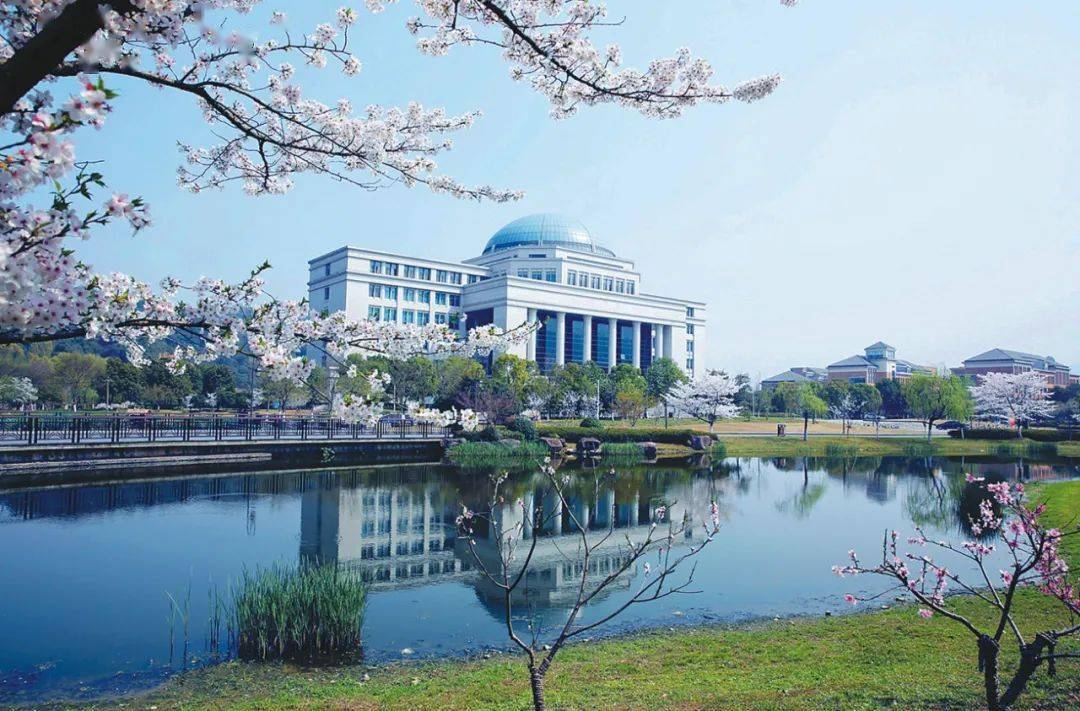
\includegraphics[width =.9\textwidth]{figures/zjut_library.jpeg}
    \caption{Zhejiang University of Technology Library}
    \label{Library}
\end{figure}

Code to insert the above image:

\begin{verbatim}
\begin{figure}[!htbp]
    \centering
    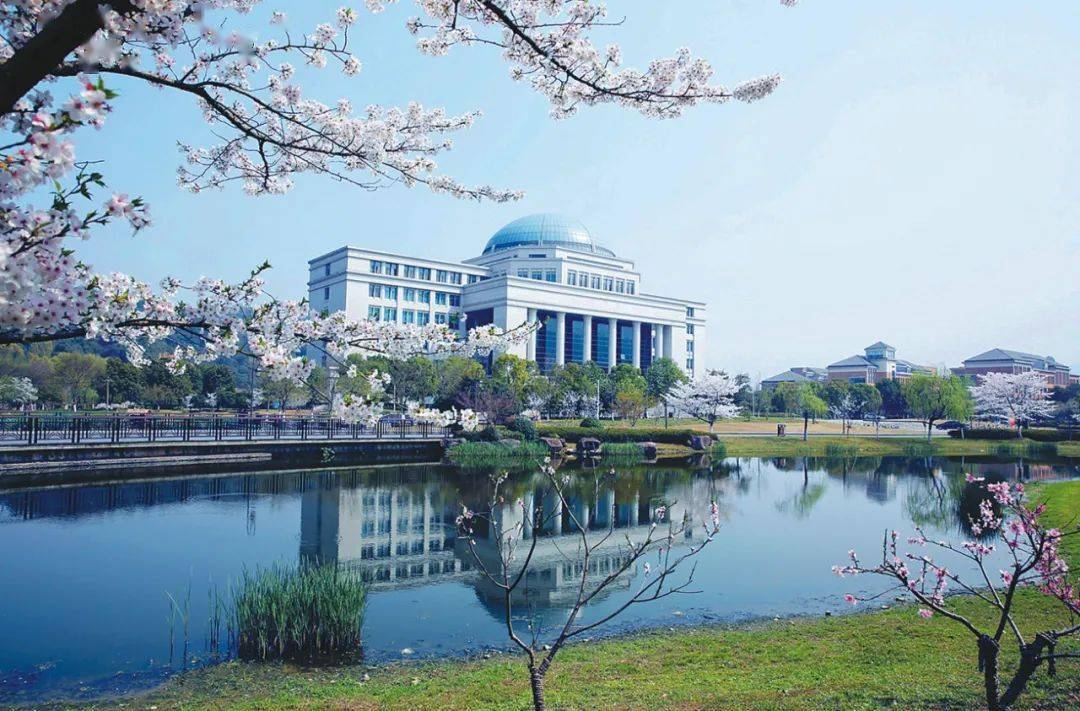
\includegraphics[width =.9\textwidth]{figures/zjut_library.jpeg}
    \caption{Zhejiang University of Technology Library}
    \label{ZJUT}
\end{figure}
\end{verbatim}

\subsection{Inserting Text Boxes}
This template defines a rounded corner gray background text box, which can be used with the simplified command \verb|\tbox{}|. If you don't like it, you can go to \texttt{ZJUTReportEN.sty} to modify it.

\tbox{
    This is a rounded corner gray background text box
}

\subsection{Inserting Tables}
The template files are shown in Table~\ref{doc}.
\begin{table}[!htbp]
    \centering
    \begin{tabular}{l  | l}
    \hline
        File Name & Description \\
        \hline
        \texttt{main.tex}  & Main file \\
        \texttt{reference.bib} & References \\
        \texttt{ZJUTReportEN.sty}  & Document format control\\
        \texttt{figures}  & Image folder \\
        \hline
    \end{tabular}
    \caption{Components of this template}
    \label{doc}
\end{table}

%\section{Theorem Environment}
%\begin{Theorem}
%\end{Theorem}
%
%\begin{Lemma}
%\end{Lemma}
%
%\begin{Corollary}
%\end{Corollary}
%
%\begin{Proposition}
%\end{Proposition}
%
%\begin{Definition}
%\end{Definition}
%
%\begin{Example}
%\end{Example}
%
%\begin{proof}
%\end{proof}

\subsection{Inserting Highlighted Code Blocks}
Using \verb|lstlisting| configuration:
\begin{lstlisting}[style=CPP, title="C++ Code"]
#include <iostream>
#include <array>
int main()
{
    constexpr int MAX = 100;
    std::array<int, MAX> arr;
}  
\end{lstlisting}

\begin{lstlisting}[style=Java, title="Java Code"]
public void addAdvertisement(String company, String ad_Category, String ad_Type, String ad_Price)
{
    int price = Integer.parseInt(ad_Price);
    ad = new Advertisement(company, ad_Category, ad_Type, price);
    adList.add(index, ad);
    index++;
    anDM = getDefaultDirectoryManager();
    ActorTuple tuple = new ActorTuple(getActorName(), "advertiser",
    company, ad_Category, ad_Type, price, index-1);
    send(anDM, "register", tuple);
}
\end{lstlisting}

\begin{lstlisting}[style=Python, title="Python Code"]                
import random
import collections
Card = collections.namedtuple('Card', ['rank', 'suit'])

class FrenchDeck:
    ranks = [str(n) for n in range(2, 11)] + list('JQKA')
    suits = 'spades diamonds clubs hearts'.split()
    
    def __init__(self):
        self._cards = [Card(rank, suit) for rank in self.ranks for suit in self.suits]
        
    def __len__(self):
        return len(self._cards)
        
    def __getitem__(self, position):
        return self._cards[position]
deck = FrenchDeck()
\end{lstlisting}

\subsection{Inserting References}
Simply use \verb|\cite{}| to cite references\cite{DBLP:conf/nips/VaswaniSPUJGKP17}.

For example:

   \textit{ Here, reference \cite{0Isaac} is cited. Reference \cite{2016The} is also cited here.}

Cited references will automatically appear in the reference section.

\section{Conclusion}
\subsection{Release Address}
\begin{itemize}
    \item GitHub: \url{https://github.com/ohhhyeahhh/ZJUT_Report_LaTeX_Template}
\end{itemize}


%%----------- References -------------------%%
% Fill in references in the reference.bib file; they will be generated automatically here

\reference


\end{document}
